\section{Theorie}
\label{sec:Theorie}
\subsection{Grundlagen der magnetischen Kernresonanz}
\label{sec:grundlagen}
Die meisten Atomkerne besitzen neben Kernladung und Masse, auch einen Eigendrehim{\-}puls, welcher als Spin $I$ bezeichnet wird.
Der Spin und das magnetische Dipolmoment des Atomkerns sind wie folgt miteinander verkn\"{u}pft:
\begin{align*}
	\overrightarrow{\mu} = \hbar \gamma \overrightarrow{I}
\end{align*}
hierbei ist $\gamma$ das gyromagnetische Verh\"{a}ltnis, welches element- und isotopenspezifisch ist.

In einem \"{a}u{\ss}eren Magnetfeld $\overrightarrow{B_0}$ richten sich die magnetischen Dipolmomente der Atomkern aus.
Klassisch betrachtet ist die Energie dann abh\"{a}ngig vom Relativwinkel zwischen $\overrightarrow{\mu}$ und $\overrightarrow{B_0}$.
In der quantenmechanischen Betrachtung sind jedoch nur bestimmte Winkel zugelasssen.
Erlaubt sind die Winkeleinstellungen, welche folgende Bedingung erf\"{u}llen:
\begin{align}
	E &= -m \hbar \gamma_I B_0  \\
	\text{mit:} \, \, \,  m &= +I, +(I-1), ..., -(I-1), -I \nonumber
\end{align}
In einem \"{a}u{\ss}eren Magnetfeld befinden sich die Atomkerne somit auf verschiedenen Energieniveaus.

Atome mit einem Kernspin von $I=\frac{1}{2}$ sind die wichtigsten Kerne für die NMR-Spektroskopie.
%- "Zeeman-Effekt"
\begin{figure}[hbtp]
	\centering
	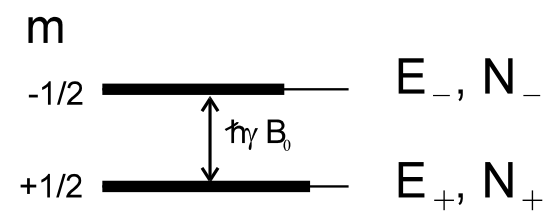
\includegraphics[width=0.5\textwidth]{Plots/energieniveaus.png}
	\caption{Aufspaltung der Energieniveaus f\"{u}r eine Atom mit Kernspin $\frac{1}{2}$ (siehe Versuchsanleitung \cite{Anleitung}[S.3]).}
	\label{Energieniveaus}
\end{figure}
In Abbildung (\ref{Energieniveaus}) ist Aufspaltung der Energieniveaus f\"{u}r solche Atome zu sehen, mit der \"{U}bergangsenergie $\Delta E = \hbar \gamma B_0$ zwischen den Niveaus.
Durch die unterschiedlichen Besetzungszahlen der einzelnen Niveaus kommt es zur makroskopischen Magnetisierung der Probe, dem sogenannten Kernmagnetismus.
%- thermodynamischen Gleichgewicht Boltzmann-Verteilung
%- Kernmoment klein -> Ausrichtung durch externes Magnetfeld, Ausrichtung ist unab\"{a}ngig von der Orientierung der Molek\"{u}le
Zus\"{a}tzlich zu der Aus{\-}richt{\-}ung kommt auf Grund des Drehimpulses eine Pr\"{a}zessionsbewegung um $\overrightarrow{B_0}$ dazu.
Die Spins pr\"{a}zedieren mit der Lamorfrequenz, $\omega_0 = \gamma B_0$.
In diesem Experiment betr\"{a}gt die Lamorfrequenz $2\pi \cdot 90 \text{\, MHz}$.
Diese Pr\"{a}zessionsbewegung ist senkrecht zum externen Magnetfeld, womit der Winkel zwischen $\overrightarrow{\mu}$ und $\overrightarrow{B_0}$ zeitlich konstant ist.
Betrachtet wird die Summe aller Kernmomente $M = \sum_i \mu_i$.
Im Gleichgewicht besitzen alle Summanden die gleiche $z$-Komponente, $M = (0,0,M_z)^{\text{T}}$.
F\"{u}r die Gesamtmagnetisierung ergibt sich
\begin{align*}
	\frac{d \mu}{d t} = \gamma \mu \times B_0
\end{align*}
Dabei sind $M$ und $B_0$ parallel zueinander und damit zeitlich konstant.
%(- M kann auch pr\"{a}zidieren)

\paragraph{Rotierendes Koordinatensystem}
Da im folgenden senkrecht zu dem konstanten Magnet\-feld ein zeitliches Hochfrequenzfeld (HF-Feld) $B_1(t)$ hinzugeschaltet wird, wird hier nun zun\"{a}chst das rotierende Koordinatensystem als Konzept eingef\"{u}hrt.
In solch einem rotierenden Koordinatensystem ergeben sich $B_0$ und $B_1(t)$ zusammen zu einem effektiven Magnetfeld $B_{eff}$.
Dreht sich die Z-Achse beispielsweise mit der Frequenz $\Omega$, siehe Abbildung (\ref{rotKoordi}a), um sich selbst, so gilt f\"{u}r die Gesamtmagnetisierung:
\begin{align*}
	\frac{dM}{dt} = \gamma M \times B - \Omega \times M = \gamma M \times \left(B - \frac{\Omega}{\gamma} \right)
\end{align*}
damit folgt f\"{u}r das effektive Magnetfeld:
\begin{align*}
	\frac{dM}{dt} = \gamma M \times B_{eff} \, \Rightarrow \, B_{eff} = B - \frac{\Omega}{\gamma}
\end{align*}
Somit wirkt das fiktive Feld $- \frac{\Omega}{\gamma}$ dem \"{a}u{\ss}eren Magnetfeld entgegen.
Das Hochfrequenzfeld wir mit einer Spule erzeugt und ist im Labor gegeben durch:
\begin{align*}
	B_1(t) = B_x cos(\Omega t)
\end{align*}
\begin{figure}[hbtp]
\caption{Rotierendes Koordinatensystem.}
\centering
	\begin{subfigure}[t]{0.35\textwidth}
	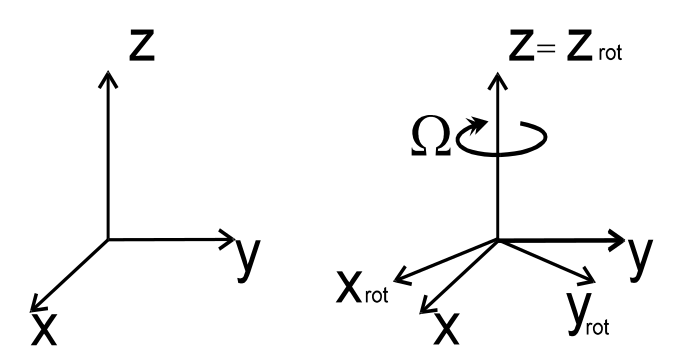
\includegraphics[width=\textwidth]{Plots/rotKoordinatensystem.png} 
	\subcaption{Die z-Achse rotiert mit Frequenz $\Omega$ (siehe Versuchsanleitung \cite{Anleitung}[S.5]).}
%	\label{rotK1}
	\end{subfigure}
	\qquad
	\qquad
	\begin{subfigure}[t]{0.35\textwidth}
	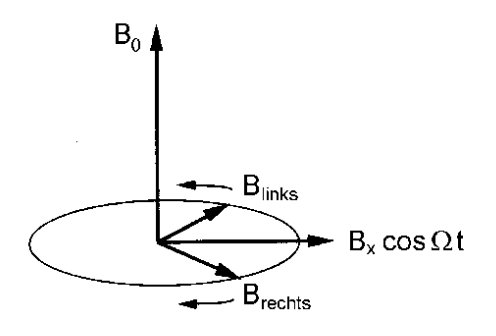
\includegraphics[width=0.8\textwidth]{Plots/B1Felder.png}
	\subcaption{Zeitabh\"{a}ngiges $B_1$-Feld wird in zwei Komponenten aufgeteilt, welche gegenl\"{a}ufig sind (siehe Versuchsanleitung \cite{Anleitung}[S.6]).}
%	\label{rotK2}
	\end{subfigure}
\label{rotKoordi}
\end{figure}
Im rotierenden Koordinatensystem wird diese HF-Feld in eine linke $B_{1,\text{links}}$ und eine rechte $B_{1,\text{rechts}}$ Komponente aufgeteilt, siehe Abbildung (\ref{rotKoordi}b).
Beide Komponenten rotieren mit einer Frequenz von $|\Omega|$ und einer Amplitude von $\frac{B_x}{2}$.
Nun kann die Komponente, die sich mit dem Koordinatensystem rotiert, als station\"{a}r betrachtet werden.
Im Gegenschluss rotiert dann die andere Komponente mit $-2\Omega$ und ist im Allgemeinen vernachl\"{a}ssigbar.

\paragraph{Die Auswirkungen von Hochfrequenzpulsen}
Um mit dem Hochfrequenzfeld, welches mit einer Spule erzeugt wird, einen Hochfrequenzpuls (HF-Puls) zu erzeugen, wird aus dem kontinuierlichen Feld der Spule ein Puls mit bestimmter L\"{a}nge herausgeschnitten,  
\setcounter{figure}{3}
\begin{figure}[hbtp]
	\centering
	\vspace{-10pt}
	\caption{Erzeugung eines HF-Pulses mit L\"{a}nge $t_p$ (siehe Versuchsanleitung \cite{Anleitung}[S.7]).}
	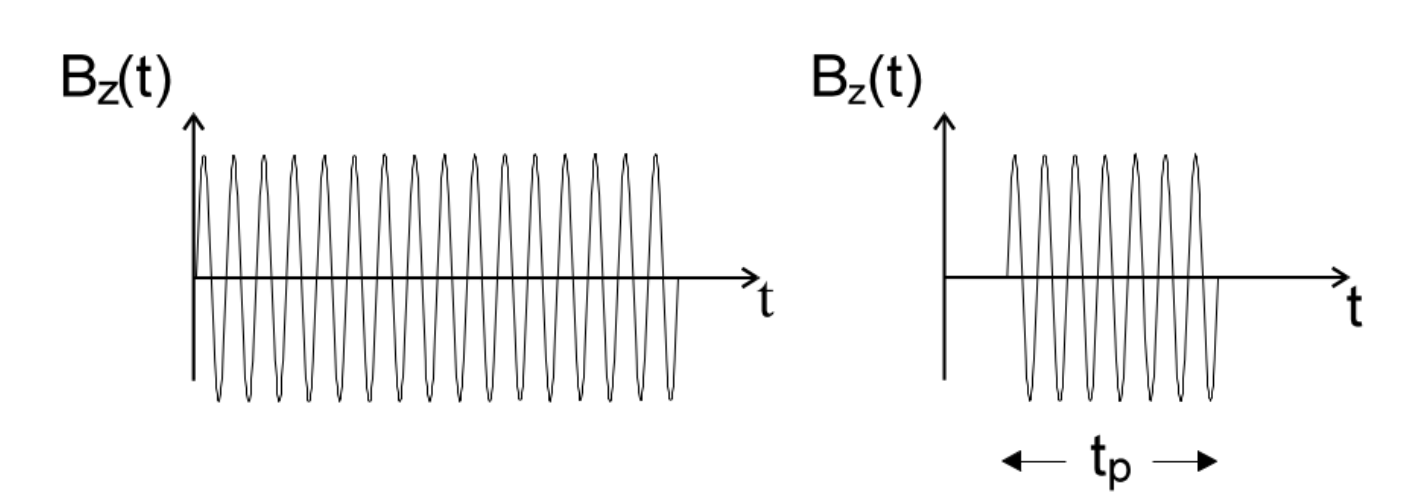
\includegraphics[width=0.55\textwidth]{Plots/HFPuls.png} 
\end{figure}
siehe Abbildung (5).
Solch ein HF-Puls wei{\ss}t genau die L\"{a}nge $t_p$ auf, dass sich die Magnetisierung um $90^{\circ}$ dreht und sich eine Quermagnetisierung einstellt.
Daher wir der HF-Puls h\"{a}ufig auch als $90^{\circ}$-Puls oder $\frac{\pi}{2}$-Puls bezeichnet.
Nachdem ein $90^{\circ}$-Puls 
\begin{wrapfigure}[15]{r}{0.5\textwidth}
	\vspace{-5pt}
	\centering
	\framebox[0.5\textwidth]{
	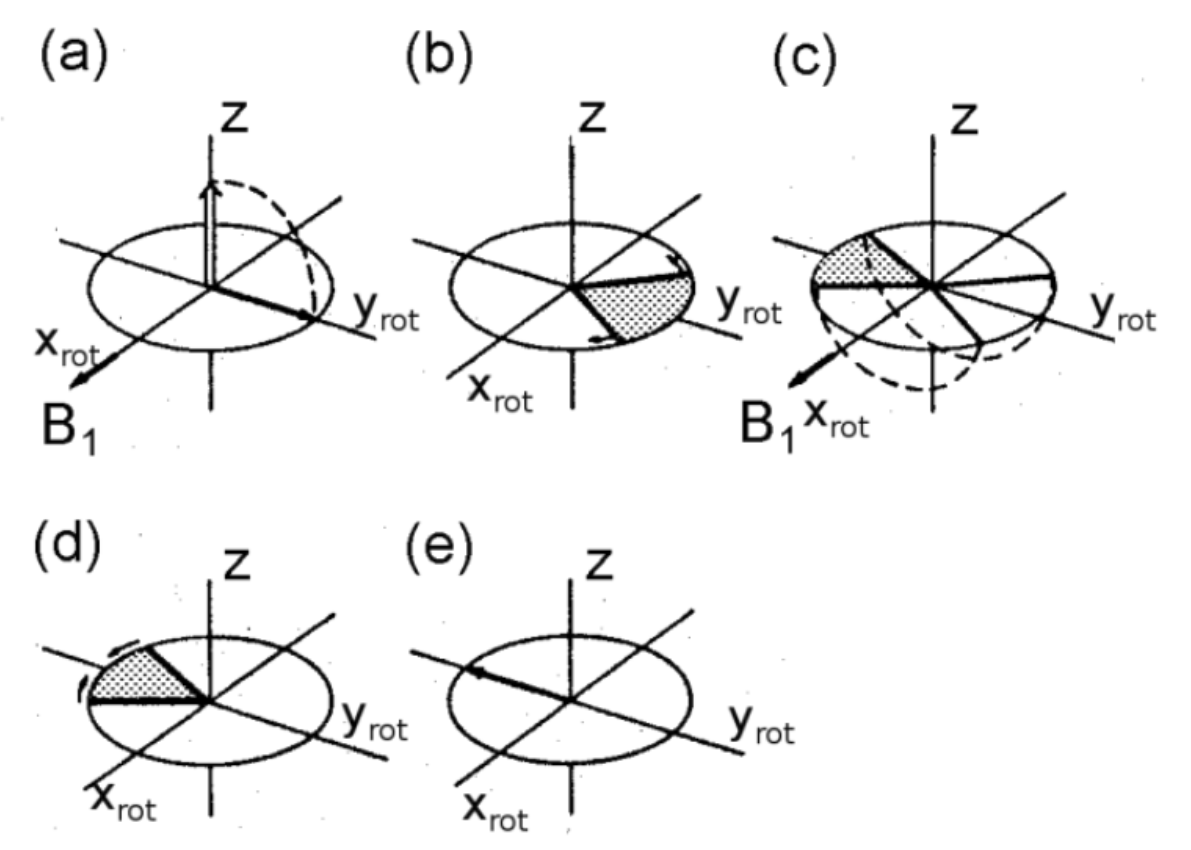
\includegraphics[width=0.45\textwidth]{Plots/hahnEcho.png} }
	\caption{Erzeugung eines Hahn-Echos durch die einen $90^{\circ}$-Puls (a) gefolgt von einem $180^{\circ}$-Puls (c) (siehe Versuchsanleitung \cite{Anleitung}[S.8]).}
	\label{HahnEcho}
\end{wrapfigure}
eingeschaltet wurde, pr\"{a}zediert die Magneti{\-}sie{\-}rung $M$ um $\overrightarrow{B_0}$.
Diese Pr\"{a}zessionsbewe{\-}gung der magnetischen Momente induziert dann eine Spannung in der Spule, in der die Probe sich befindet.
Es wird ein Kerninduktionssignal erzeugt.
Gemessen wird der Momentanwert der L\"{a}ngsmagnetisierung.
Die durch den $90^{\circ}$-Puls erzeugte Quermagnetisierung wird mit der Zeit kleiner, da die effektive Quermagnetisierung anf\"{a}ngt zu dephasieren, siehe Abbildung (\ref{HahnEcho}b).
Der Zerfall der Quermagnetisierung wird auch als freier Induktionszerfall bezeichnet und mit FID (\textbf{F}ree \textbf{I}nduction \textbf{D}ecay) abgek\"{u}zt.
Durch einen danach eingeschalteten $180^{\circ}${\-}Puls kommt es zur Rephasierung der Dipol{\-}mo{\-}men{\-}te (Abbildung (\ref{HahnEcho}d)).
Das Zusam{\-}men{\-}tref{\-}fen der Signalpunkte (Abbildung (\ref{HahnEcho}e)) wird als Hahn-Echo bezeichnet und kann gemessen werden.
Bisher wurden die Wechselwirkungen zwischen den Spins und ihrer Umgebung noch nicht betrachtet.
Sowohl durch rotatorische, als auch durch translatorische Molekularbewegung zerf\"{a}llt die Magnetisierung irreversible
Daher ist zu beachten, dass die Magnetisierung im Hahn-Echo nicht der Magnetisierung nach dem $90^{\circ}$-Puls entspricht.


\subsection{Relaxationen}
Die Magnetisierung $M(t)$ welche nach einen HF-Puls in der Probe vorliegt strebt wieder den Gleichgewichtswert $M_{eq}$ an.
Die Relaxation der Magnetisierung beruht auf der Wechselwirkung zwischen den Spins und deren Umgebung und wird in zwei Komponenten geteilt.
Zum Einen die longitudinale Relaxation entlang der z-Achse
\begin{align}
	\frac{d M_z(t)}{d t} = - \frac{M_z(t) - M_{eq}}{T_1} 
	\label{eq:bloch1}
\end{align}
und zum Anderen die transversale Relaxation in der x,y-Ebene
\begin{align}
	\frac{d M_{x,y}(t)}{d t} = - \frac{M_{x,y}(t)}{T_2}. 
	\label{eq:bloch2}
\end{align}
Diese beiden Gleichungen \eqref{eq:bloch1} und \eqref{eq:bloch2} sind als die Bloch-Gleichungen bekannt.
Dabei ist $T_1$ die Spin-Gitter-Relaxationszeit und $T_2$ die Spin-Spin-Relaxationszeit.
Im folgenden wird n\"{a}her auf die beiden Relaxationen eingegangen.

\paragraph{Spin-Gitter-Relaxation}
Die longitudinale Relaxation wird auch als Spin-Gitter-Relaxa{\-}tion bezeichnet.
Um die Spin-Gitter-Relaxation mikroskopisch zu beschreiben, werden die verschiedenen Energieniveaus betrachtet, wie in Abbildung (\ref{Energieniveaus}) zu sehen.
Durch einen $180^{\circ}$-Puls folgt eine Besetzungszinversion in den energetisch ung\"{u}nstigeren Zustand.
Die Spin-Gitter-Relaxationszeit $T_1$ beschreibt nun die Zeit, die ben\"{o}tigt wird, bis das Spinsystem wieder im Gleichgewichtszustand ist.
Somit beschreibt $T_1$ wie schnell  die Spins in den energetisch g\"{u}nstigen Zustand \"{u}bergehen.
%- spontane \"{U}berg\"{a}nge sehr unwahrscheinlich
%- Emissionsprozesse m\"{u}ssen induziert werden -> durch magnetisches Wechselfeld
Diese \"{U}berg\"{a}nge m\"{u}ssen nicht durch ein externes Wechselfeld induziert werden.
Denn die rotatorische und translatorische Bewegung der Spins erzeugen selber ein Wechselfeld, wodurch die \"{U}berg\"{a}nge geschehen.
Einhergehend mit diesen \"{U}berg\"{a}ngen ist ein Fluss von Energiequanten $(\hbar \omega_0)$ zwischen Kernspinsystem und Gitter.
Jedoch ist der Energiequantenfluss relatiiv klein.

Die dazugeh\"{o}rige $T_1$ Zeit kann mit der Inversionserholung gemessen werden.
Hierbei folgt auf einen $180^{\circ}$-Puls ein $90^{\circ}$-Puls.
In Abbildung (\ref{inversion}) ist diese Pulssequenz schematisch gezeigt.
\begin{SCfigure}[1][!h]
	\centering
	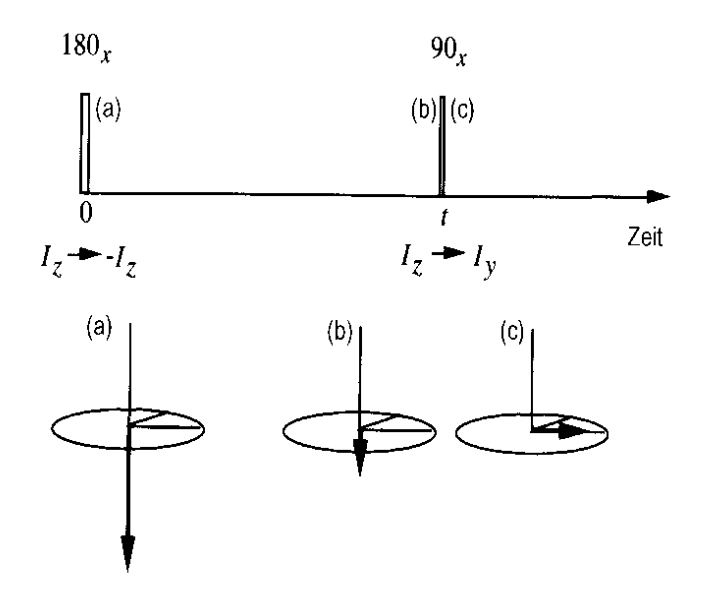
\includegraphics[width=0.5\textwidth]{Plots/inversionserholung.png}
	\caption{Oben die Pulssequenz f\"{u}r eine Inversionserholung zur Messung der $T_1$-Zeit. Darunter ist die dazugeh\"{o}rige Magnetisierung veranschaulicht (siehe Versuchsanleitung \cite{Anleitung}[S.10]).}
	\label{inversion}
\end{SCfigure}
Nach den zwei eingeschalteten Pulsen zerf\"{a}llt die erzeugte Quer{\-}mag{\-}ne{\-}ti{\-}sie{\-}rung wieder und ein FID-Signal ist messbar.
Da die Amplitude dieses Signals proportiuonal zu der longitudinalen Magnetisierung ist, kann daraus dann die Relaxationszeit $T_1$ bestimmt werden.
Zus\"{a}tzlich dazu kann aus der ersten Blochgleichung die zeitabh\"{a}ngige longitudianle Magnetisierung ermittelt werden.
\begin{align*}
	M_z(t) = M_{eq} \left(1 - 2 exp\left( - \frac{t}{T_1} \right) \right)
\end{align*}
Um eine grobe Absch\"{a}tzung der longitudinalen Relaxationszeit vorzunehmen, kann folgende Gleichung verwendet werden:
\begin{align*}
	t_{\frac{1}{2}} = T_1 \cdot ln(2) \, \Rightarrow \, M_z(t) = 0
\end{align*}
Solch eine Absch\"{a}tzung ist wichtig, da sichergestellt werden soll, dass jede neue Messung wieder mit im Gleichgewichtszustand starten soll.
Um dies zu gew\"{a}hrleisten sollt zwischen zwei Messungen eine Wartezeit von $t \approx 4 \cdot T_1$ sein.
Dadruch wird auch das Sihnal-zu-Rauch-Verh\"{a}ltnis verbessert.

Neben der Inversionserholung gibt es noch die M\"{o}glichkeit mittels einer S\"{a}ttigungs{\-}erhol{\-}ung die $T_1$-Zeit du bestimmen.
Hierbei wird zun\"{a}chst die Magnetisierung duch zuf\"{a}llig hintereinander geschaltete Pulse zerst\"{o}rt.
Durch den Wideraufbau der L\"{a}ngmagnetisierung kann dann die $T_1$-Zeit bestimmt werden.

\paragraph{Spin-Spin-Relaxation}
%\begin{wrapfigure}[12]{r}{0.35\textwidth}
%	\centering
%	\vspace{-10pt}
%	\framebox[0.3\textwidth]{
%	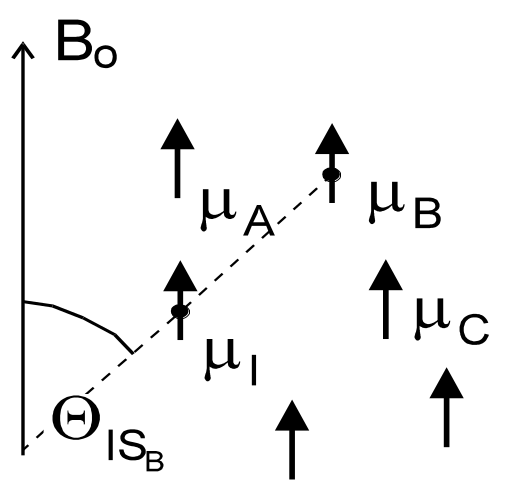
\includegraphics[width=0.25\textwidth]{Plots/spin_spin.png} }
%	\caption{Schematische Darstellung der Spin-Spin-Wechselwirkung (siehe Versuchsanleitung \cite{Anleitung}[S.12]).}
%	\label{SpinSpin}
%\end{wrapfigure}
Die zweite Relaxation be{\-}ruht auf der Spin-Spin-Wechselwirkung, welche auch als magnetische Wechselwirkung zwischen den Dipolen aufgefasst werden kann.
Und anders als bei der Spin-Gitter-Relaxation flie{\ss}t hierbei kein Energiefluss ins Gitter.
Durch die Wechselwirkung zwischen den Spins ist die St\"{a}rke der Zusatzfelder abh\"{a}ngig von dem Winkel, $\vartheta$, zwischen $B_0$ und $r$ (Abbildung (\ref{SpinSpin})).
\begin{SCfigure}[1][!h]
	\centering
	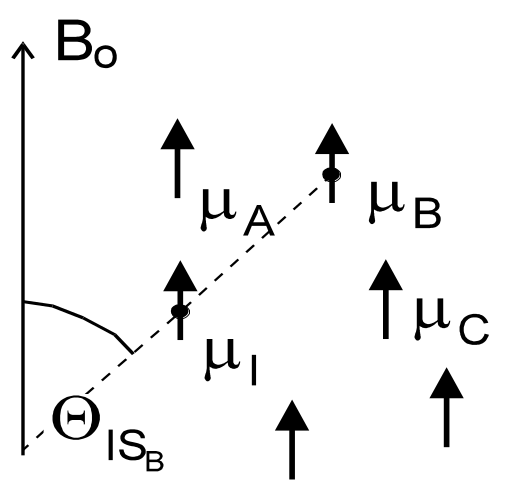
\includegraphics[width=0.25\textwidth]{Plots/spin_spin.png}
	\caption{Schematische Darstellung der Spin-Spin-Wechselwirkung (siehe Versuchsanleitung \cite{Anleitung}[S.12]).}
	\label{SpinSpin}
\end{SCfigure}
Mathematisch ergeben sich die Zusatzfelder der Nachbarspins zu:
\begin{align*}
	B_z^{DD} &= \sum_s \hbar \gamma_s S \left( 3 cos^2 \left(\vartheta_{IS}\right) - 1 \right) \frac{1}{r_{IS}^3} \\
	\text{und} \, \, \, \, B_{x,y}^{DD} &= \sum_s \hbar \gamma_s S \left( \frac{3}{2} \cdot sin\left(2 \vartheta_{IS}\right) \right) \frac{1}{r_{IS}^3} 
\end{align*}

Im Vergleich zu $T_1$-Relaxationszeit ist die Spin-Spin-Relaxationszeit $T_2$ in Festk\"{o}rpern immer kleiner.
Nur in Fl\"{u}ssigkeiten sind beide Relaxationszeiten in dergleichen Gr\"{o}{\ss}en{\-}ord{\-}nung.

\subsection{Der Kernspin des Deuterons}
Befindet sich ein Atomkern in einem externen Magnetfeld so spalten sich die Energie{\-}ni{\-}veaus.
Dieser Effekt ist auch unter dem Namen Zeeman-Effekt bekannt.
Anders als die bisher behandelten Atomkerne hat das Deuteron einen Spin von $I = 1$.
Zus\"{a}tzlich besitzt das Deuteron auch ein elektrisches Quadrupolmoment.
\begin{figure}[hbtp]
	\centering
	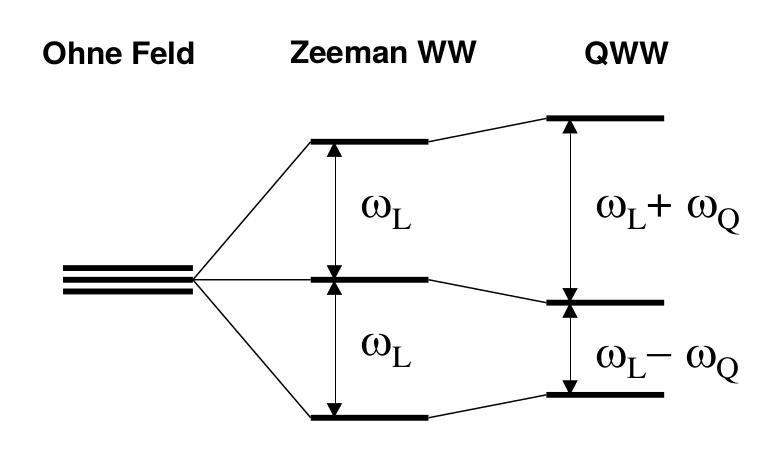
\includegraphics[width=0.4\textwidth]{Plots/aufspaltung.png}
	\caption{Aufspaltung der Energieniveaus im externen Magnetfeld unter ber\"{u}cksichtigung der Zeeman- und Quadropol-Wechselwirkung (siehe Versuchsanleitung \cite{Anleitung}[S.19]).}
	\label{QWW}
\end{figure}
Im externen Magnetfeld muss nun also nicht nur die Zeeman-Wechselwirkung, sondern auch die Quadropol-Wechselwirkung ber\"{u}cksichtigt werden, da das Quadropolmoment mit dem elektrischem Feldgradienten wechselwirkt.
Dadurch verschieben sich sich die Energieniveaus, siehe Abbildung (\ref{QWW}).
Zu sehen ist, dass sich der Abstand zwischen den Energieniveaus einmal um $\omega_Q$ vergr\"{o}{\ss}ert und einmal verkleinert.

\subsection{Echo-Signale in der NMR}
In der Festk\"{o}rper-NMR ist die Dephasierung der Spins oft auf Grund der breiten Frequenzspektren sehr schnell.
Um eine Rephasierung der Spins, und somit ein Echo-Signal, herbeizuf\"{u}hren und die sonst sehr kurze Beobachtungszeit zu \"{u}berwinden, wird ein zweiter HF-Puls verwendet.
Zwischen den beiden Pulsen sollte die Wartezeit der Totzeit entsprechen, um sicherzustellen, dasss die Spins wieder in Phase gebracht werden.
Im Folgenden werden zwei % bzw drei
Echo-Signale n\"{a}her erl\"{a}utert.

\paragraph{Hahn-Echo}
Wie schon in Kapitel (\ref{sec:grundlagen}) erw\"{a}hnt, wird das Hahn-Echo mit einem $90^{\circ}$- und einem $180^{\circ}$-Puls erzeugt.
Auf Grund von Inhomogenit\"{a}ten im Magnetfeld rephasieren die Spins nach dem $90^{\circ}$-Puls, da die Spins mit unterschiedliecher Lamorfrequenz pr\"{a}zedieren.
Wie in Abbildung (\ref{HahnEcho} b) zu sehen, laufen Spins mit schnellerer und langsamerer Lamor{\-}fre{\-}quenz auseinander.
Durch den dahinter geschalteten $180^{\circ}$-Puls werden die Spins so gedreht, dass sie nun alle auf einem Punk zusammentreffen und ein Echo erzeugen.

Das Hahn-Echo wird meist f\"{u}r die Refokussierung von Wechselwirkungen verwendet, welche linear in $\widehat{I}_z$ sind.
%- zum Beispiel: chemische Verschiebung, Dipol-Dipol-Wechselwirkung, Inhomogenit\"{a}ten von $B_{ext}$
%-> mit $\widehat{H}_z = \omega \widehat{I}_z$

\paragraph{Festk\"{o}rper-Echo}
Das Festk\"{o}rper-Echo wird durch eine Pulssequenz von zwei aufeinan{\-}der folgenden $90^{\circ}$-Pulsen verwendet, welche um $\frac{\pi}{2}$ zueinander phasenverschoben sind, erzeugt.
Das zweiten $90^{\circ}$-Puls dient hierbei zur Refokussierung der gegenseitigen magne{\-}tisch{\-}en Dipol-Dipol-Wechselwirkung der Kerne im Festkörper.
%welche bilinear in homonuklearen Spinoperatoren sind.
Wird dieser zweite Puls zur Zeit $t_p$ eingestrahlt, so folgt die Rephasierung der Spins zum Zeitpunkt $2 t_p$.
Mit dem Festk\"{o}rper-Echo kann somit der Informationsverlust w\"{a}hrend der Totzeit umgangen werden.
\begin{SCfigure}
\centering
	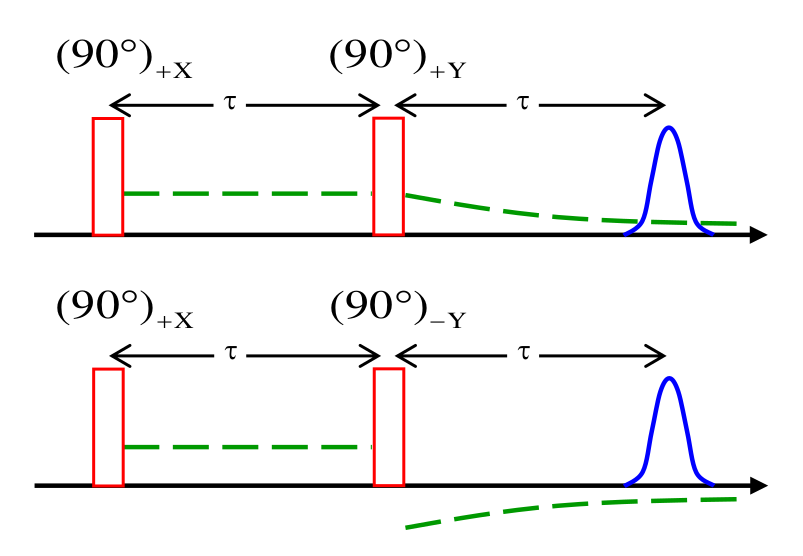
\includegraphics[width=0.4\textwidth]{Plots/festkoerperecho2.png}
%	\includegraphics[width=0.4\textwidth]{Plots/FK_Echo_diss.png}
	\caption{Zwei verschiedene Pulssequenzen zur Erzuegung eines Festk\"{o}rper-Echos. Die Variable $\tau$ in der Abbildung entspricht der Zeit $t_p$ (siehe Versuchsanleitung \cite{Anleitung}[S.18]).}
	\label{FK_echo.}
\end{SCfigure}
In Abbildung (\ref{FK_echo.}) ist die Pulssequenz f\"{u}r solch ein Festk\"{o}rper-Echo schematisch aufgezeicht.
Zu sehen ist dort auch, dass es f\"{u}r das erzeugte Echo keinen Unterschied macht, ob der zweite Puls eine Rotation um die $+Y$- oder $-Y$-Achse ausf\"{u}hrt.
Lediglich das Vorzezichen des FID h\"{a}ngt von der Phase des zweiten Pulses ab.

\subsection{Stimuliertes Echo}
Ist es nun erw\"{u}nscht sehr langsame Prozesse zu studieren, so ist es sinnvoll die Dephasie{\-}rung von der Rephasierung zu trennen.
Dies kann mit dem stimulierten Echo erreicht werden.
Daf\"{u}r wird bei einer Pulssequenz der zweite HF-Puls aufgeteilt.
Die Zeit zwischen dem dann zweiten und dritten Puls ist die sogenannte Mischzeit $t_m$.
\begin{figure}
\centering
\caption{Stimuliertes-Echo.}
\vspace{+5pt}
	\begin{subfigure}[t]{0.4\textwidth}
		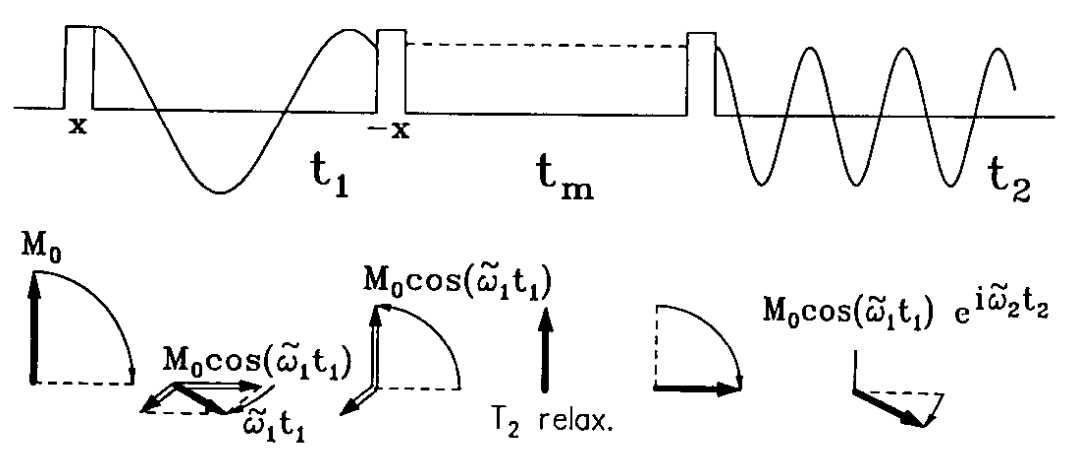
\includegraphics[width=\textwidth]{Plots/stimuliertesecho.png} 
		\caption{Schematische Pulssequenz des Stimulierten-Echos mit zugeh\"{o}riger Magnetisierung (siehe Versuchsanleitung \cite{Anleitung}[S.21]).}
%		\label{stimEcho_a.}
	\end{subfigure}
	~
	\begin{subfigure}[t]{0.4\textwidth}
		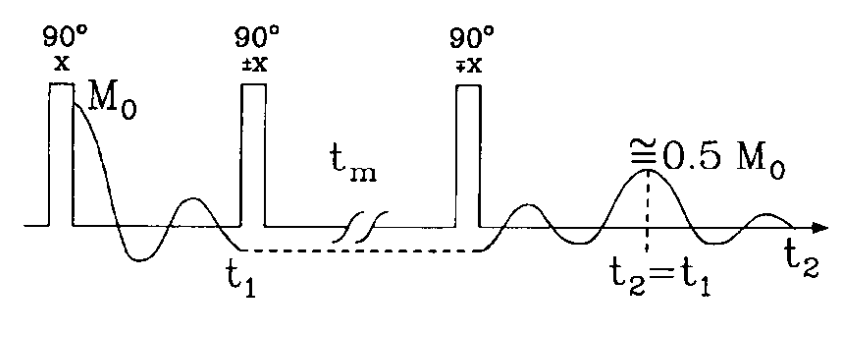
\includegraphics[width=\textwidth]{Plots/stimuliertesecho2.png}
		\caption{Die Magnetisierung des Echo-Signal ist beim Stimulierten-Echo nur halb so gro{\ss} wie die anf\"{a}ngliche Magnetisierung(siehe Versuchsanleitung \cite{Anleitung}[S.24]).}
%		\label{stimEcho_b.}
	\end{subfigure}
\label{stimEcho.}
\end{figure}
Anschaulich sind die drei HF-Pulse in Abbildung (\ref{stimEcho.}a) zu sehen.
Mit dem ersten Puls wird die transversale Magnetisierung hergestellt, welche bekanntlich w\"{a}hrend der $t_1$ Zeit dephasiert.
Nun kann mit dem zweiten Puls die cos- oder sin-Komponente ausgew\"{a}hlt werden.
Diese ausgew\"{a}hlte Komponente wird zur\"{u}ck in die z-Richtung gedrehtund somit in die langlebige longitudinale Magnetisierung gebracht, welche nur noch mit $T_2$ zerf\"{a}llt.
Der zweite Puls wird daher auch oft als Scheicherpuls bezeichnet.
Erf\"{u}llt die Mischzeit $t_m$ folgende Bedingung: $T_2 \ll t_m \ll T_1 $, so dephasiert die Quermagnetisierung, welche vom Speicherpuls unber\"{u}hrt in der xy-Ebene verblieben ist.
Mittels des dritten $90^{\circ}$-Pulses wird die gespeicherte Magnetisierung abgerufen und kann nach der Zeit $t_1 = t_2$ als Stimuliertes-Echo gemessen werden.
Die Magnetisierung des Echos ist dabei nur halb so gro{\ss}, siehe Abbildung (\ref{stimEcho.}b).
%\begin{figure}[hbtp]
%	\centering
%	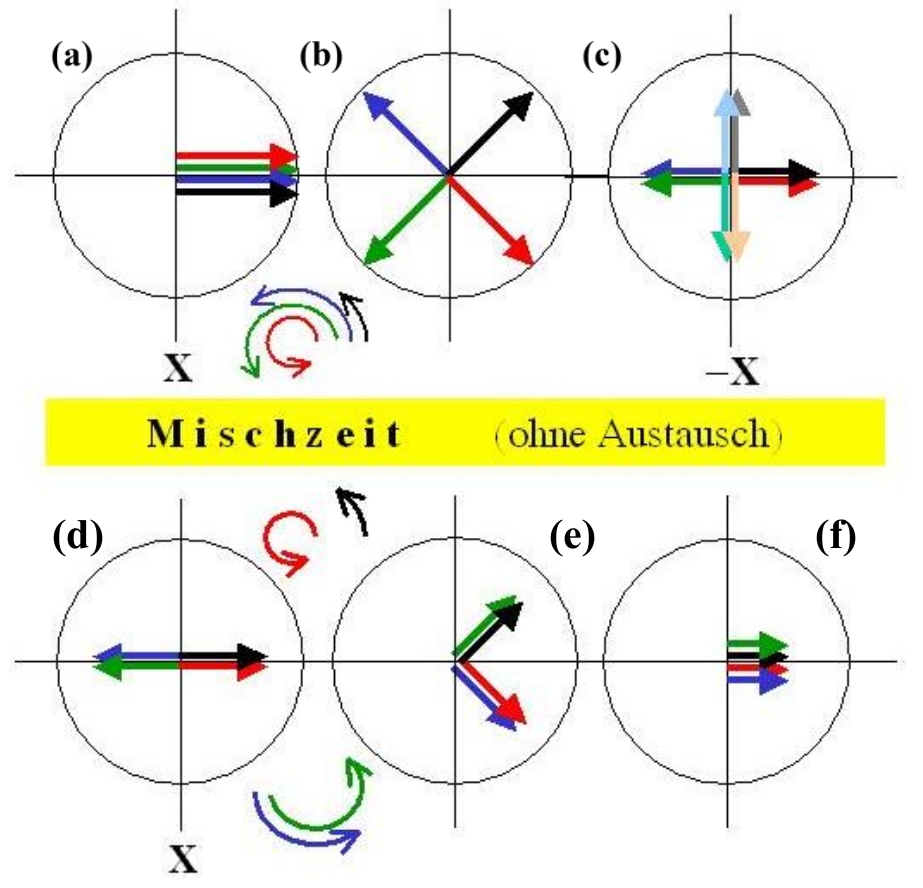
\includegraphics[width=0.5\textwidth]{Plots/mischzeit.png}
%	\caption{.}
%	\label{.}
%\end{figure}
